\chapter{Abstract Syntax Metamodels}
\label{abschapter}

\section{Introduction}

Just as a the quintessential step in object oriented design is constructing a model of system concepts, constructing an abstract syntax metamodel is an essential first step in the design of a modelling language. An abstract syntax metamodel describes the concepts in the language and their relationships to each other. In addition, it also defines the rules that determine whether a model written in the language is valid or not. These are the well-formedness rules of the language. 

Imagine a business modelling language suitable for modelling high level business rules about business data. An appropriate language for this domain might provide modelling concepts such as "data model", "data entity", and "business rule". In addition, there will be relationships between these concepts: a "data model" may be composed of a number of "data entities". There will also be rules describing the valid models that may be constructed in the language, for instance, "a datamodel cannot contain two or more data entities with the same name" might be one such rule. 

The concepts, relationships and rules identified during this step will provide a vocabulary and grammar for constructing models in the language. This will act as a foundation upon which all other artefacts of the language design process will be rooted.  

This chapter describes the steps required to construct abstract syntax metamodels, along with examples of their application to the definition of the abstract syntax model of a simple modelling language. 

\section{Modelling Abstract Syntax}

As stated, the purpose of an abstract syntax metamodel is to describe the concepts in a language and the relationships that exist between those concepts. In the context of a language definition, a concept is anything that represents a part of the vocabulary of the language. The term abstract syntax emphasises a focus on the the abstract representation of the concepts, as opposed to the notation of the concepts or their semantics. As a result, abstract syntax metamodels tend to focus on the static, syntactical properties of concepts in a language. Note that it is not the purpose of the abstract syntax metamodel to describe the semantics of the language, or how it will be presented. These aspects will be described later.

In addition, an abstract syntax metamodel should also describe the rules by which a model written in the language is deemed to be well-formed, i.e. is syntactically valid. These provide a more detailed description of the syntactical rules of the language than is possible just by describing the concepts and relationships alone. These well-formedness rules are particularly useful when it comes to implementing a tool to support the language, as they can be used to validate the correctness of models as they are created.

Constructing an abstract syntax metamodel has much in common with developing an abstract grammar for a programming language, albeit that the language used is more expressive than that used in programming language design. 

Abstract syntax metamodels are written in a metamodelling language. As described in chapter \ref{xmofchapter}, the metamodelling language we will use, called XMOF, provides a number of modelling abstractions suitable for modelling languages. For the purposes of modelling abstract syntax, only a subset of XMOF will be required. This is the subset suitable for capturing the static properties of language concepts and rules of well-formedness, and includes:

\begin{itemize}
\item classes to describe the concepts in the language;
\item packages to partition the metamodel into manageable chunks where necessary.
\item attributes and associations to describe the relationships between concepts;
\item constraints, written in OCL, to express the well-formedness rules.
\end{itemize} 

\section{The Process}

There are a number of stages involved in developing an abstract syntax metamodel: concept identification; concept modelling; model architecting; model validation and model testing. These stages are described below.

\subsection{Concept Identification}
\label{conceptidentification}

The first stage in modelling the abstract syntax of a language is to utilise any information available to help in identifying the concepts that the language uses, and any obvious rules regarding valid and invalid models. 

There are a number of useful techniques that can be used to help in this process:

\begin{itemize}

\item Construct a list of candidate concepts in the language. Focus on determining whether the concepts make sense as part of the language's vocabulary. In particular, identify concepts that match the following criteria:

\begin{itemize}
  \item Concepts that have names.
   \item Concepts that contain other concepts, e.g. a class containing attributes.
  \item Concepts that record information about relationships with other concepts, e.g. named associations between classes.
  \item Concepts that play the role of namespaces for named concepts.
  \item Concepts that exhibit a type/instance relationship.
  \item Concepts that are recursively decomposed.
  \item Concepts that are a part of an expression, or which are associated with expressions.
\end{itemize}

\item Build examples of models using the language. 

\begin{itemize}
\item Utilise any notation that you think appropriate to represent each type of concept. Use this notation to build models of meaningful/real world examples. 
\item In the case of a pre-existing language there should be examples already available to help in the identification of concepts. Other good sources of inspiration include CASE tools, which will provide automated support for building example models. Such tools may also provide additional facilities for checking valid and invalid models, which will be useful when identifying well-formedness rules or may provide more detailed examples of the language syntax. 
\end{itemize}
 
\end{itemize}

Once some examples have been constructed, abstract away from them to identify the generic language concepts and relationships between concepts. It is often useful to annotate the examples with the modelling concepts as a precursor to this step. Examples of invalid models can also be used to help in the identification of well-formedness rules. 

It is important during this process to distinguish between the concrete syntax of a language and its abstract syntax. Whilst it is common for the structure of the abstract syntax to reflect its concrete syntax, this need not be the case. For example, consider a language which provides multiple, overlapping views of a small number of core modelling concepts. In this case, the abstract syntax should reflect the core modelling concepts, and not the concrete syntax. 

'Modelling the diagrams' is a common mistake made by many novice metamodellers. If in doubt, ask the following questions when identifying concepts:

\begin{itemize}
\item Does the concept have meaning, or is it there purely for presentation? If the latter, then it should be viewed as concrete syntax. An example might be a "Note", which clearly does not deserve to be modelled as an abstract syntax concept.
\item Is the concept a derived concept, or is it just a view on a collection of more primitive concepts? If so, a relationship should be defined between the richer concept and the more primitive concept. Consider a dataflow between a process and a datastore that is derived from the fact that the process has an action that updates the datastore. 
\end{itemize}

In general, the best abstract syntax models are the simplest ones. Any complexity due to diagrammatical representation should be deferred to the concrete syntax models.

\subsection{Concept Modelling}

Once concepts have been identified, standard OO modelling features, classes, packages, and associations are applied to model the concepts in the language. There are many examples of developing conceptual models available in the literature, for instance, \cite{Larman} devotes a significant amount of time to this subject. 

In general, concepts will be described using classes, with appropriate attributes used to capture the properties of the concepts. Some concepts will have relationships to other concepts, and these will be modelled as associations. Where it makes sense to define categories of concepts, generalization can be used to seperate them into more general and more specific types of concepts.

A useful strategy to apply at this stage is to reuse existing language definitions where possible. There are a number of techniques that can be used to achieve this, including:

\begin{itemize}
\item Extending or tailoring an existing metamodel to fit the new language. This can be achieved by specializing classes from the existing metamodel or by using package extension to import and extend whole packages of concepts.
\item Utilising language patterns. A language pattern may be realised as a framework of abstract classes that capture a repeatedly used language structure, or by a package template (a parameterized package).
\end{itemize}

\noindent A full discussion of these techniques will be presented in chapter ??.

\subsection{Well-formedness Rules and Operations}

Once a basic metamodel has been constructed, start identifying both legal and illegal examples of models that may be written in the language. Use this information to define a set of well-formedness rules in XOCL that rule out the illegal models. When defining rules, look to identify the most general rules possible, and investigate the implications of what happens when rules are combined - sometimes rules can conflict in unexpected ways. There are many books available on writing constraints in OCL that can help guide this process, see \cite{Warmer} for example. Reusing existing language components can also minimise the effort involved in writing well-formedness rules, as constraints can be reused as well - however, be aware that if specialisation is used then.

Operations and queries should also be defined where appropriate. Examples of operations include general utility operations such as creating new model elements and setting attribute values, or operations that act as test harnesses. Examples of queries might include querying properties of models for use in constraints and operations, or for validation purposes. Operations that change the state of models should take into account any constraints, ensuring that if a constraint holds before the operation is invoked, it will continue to hold afterwards.

\subsection{Use Cases}

A very useful technique to understanding and defining the properties of a modelling language is to consider the different use cases associated with using the language. This is almost akin to writing a metamodel API, i.e. a collection of operations that would be used when interacting with the metamodel. Some typical use cases might include creating and deleting model elements, but may also include semantically rich operations such as transforming a model, or executing a statemachine. Taken to its extremes, such an approach can be used to completely drive the identification of concepts in a metamodel: in effect a use case driven approach. However, as is always a case, an iterative process is always useful.

\subsection{Metamodel Integration}

At some point during the development of the abstract syntax model, it will need to be integrated within a specific metamodelling framework. This will enable it to take advantage of the generic mechanisms and APIs provided by the framework and will support its implementation in a tool. The XMOF framework provides generic mechanisms that includes model element instantiation, parsing and expression evaluation. Thus, an analysis of where the classes in the abstract syntax model need to extend or reference classes in the framework should be undertaken.

%More required here.

\subsection{Validation and Testing}

It is important to validate the correctness of the abstract syntax model. Investing in this early on will pay dividends in the longer run. A useful (static) technique for doing this is to construct instances of the abstract syntax metamodel that match those of example models. An object diagram is a useful way of capturing this information as it shows instances of classes (objects) and associations (links). There are tools available that will both help create object diagrams, and also check they are valid with respect to a model and any OCL constraints that have been defined. 

The best means of testing the correctness of a language definition is to build a tool that implements it. Only then, can the language be tested by end users in its entirety. Tools that facilitate the rapid generation of tools from metamodels are discussed in more detail in chapter ??.

\section{Case Study}

The best way to learn about metamodelling is to look at some real examples. An example of a simple, but widely known modelling language, is a data flow diagram, or DFD. DFD's were widely used in the 1980's and early 1990's as a notation for modelling the flow of data between entities in a system. Indeed they are still used today by data modellers as an important tool for eliciting data structures. DFD's are a good starting point for illustrating metamodelling as they are simple, but illustrated many facets of the metamodelling process.

As shown in figure \ref{dfdexample}, a DFD is essentially a visual network of data flows between processes, data stores and external entities, which aims to model the logical flow of data in a system and the transformations that occur to the data (without committing to physical implementation details). 

\begin{figure}[htb]
\begin{center}
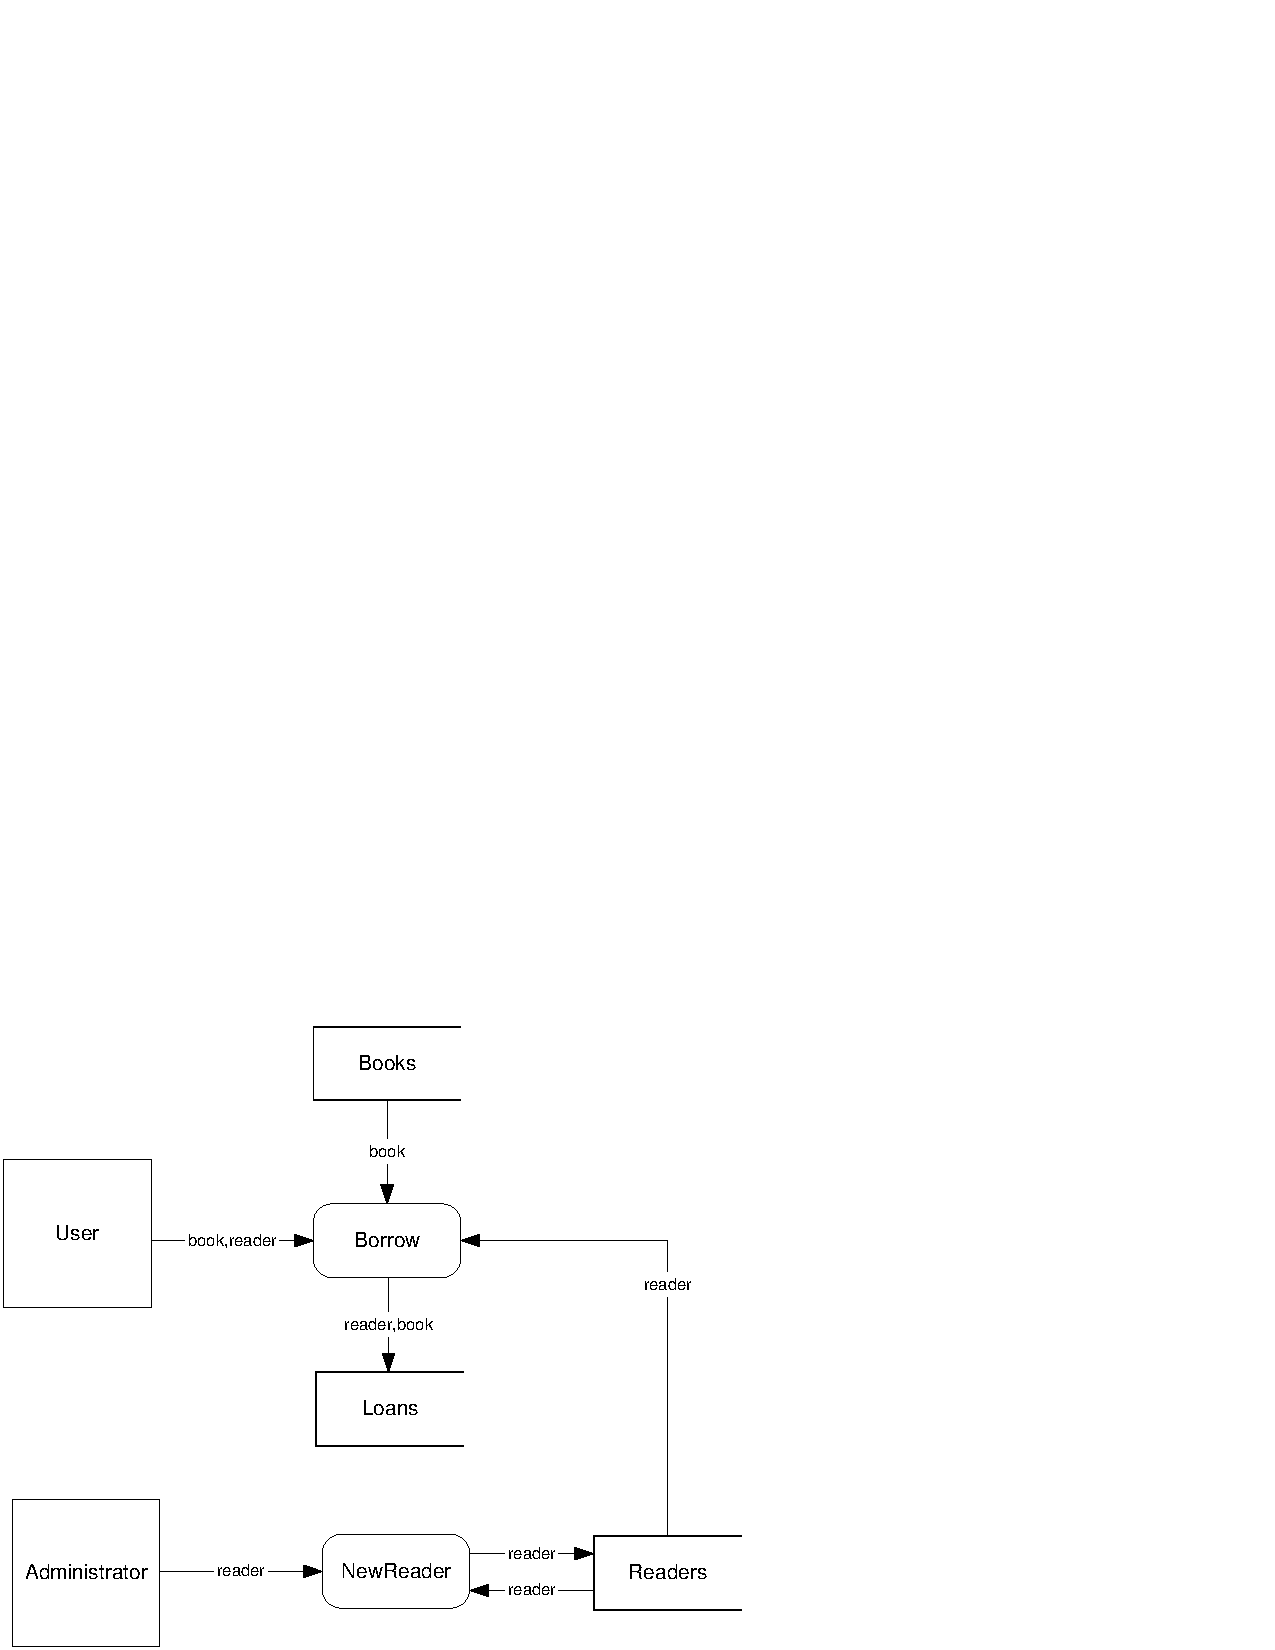
\includegraphics[width=13cm]{AbstractSyntax/figures/DFDExample.pdf}
\caption{An example of a data flow diagram (DFD)}
\label{dfdexample}
\end{center}
\end{figure}

There are a number of other features of DFDs that are not illustrated by this example. One of the most important is the ability for processes to be nested. As shown in figure \ref{dfdnested} ,this enables a single process node on a high level diagram to be expanded to show a more detailed collections of processes. The highest level process in the DFD hierarchy is commonly called a context diagram. This provides a view of the system as a single process, along with the input and output dataflows that flow to and from the external entities to the system.

\begin{figure}[htb]
\begin{center}
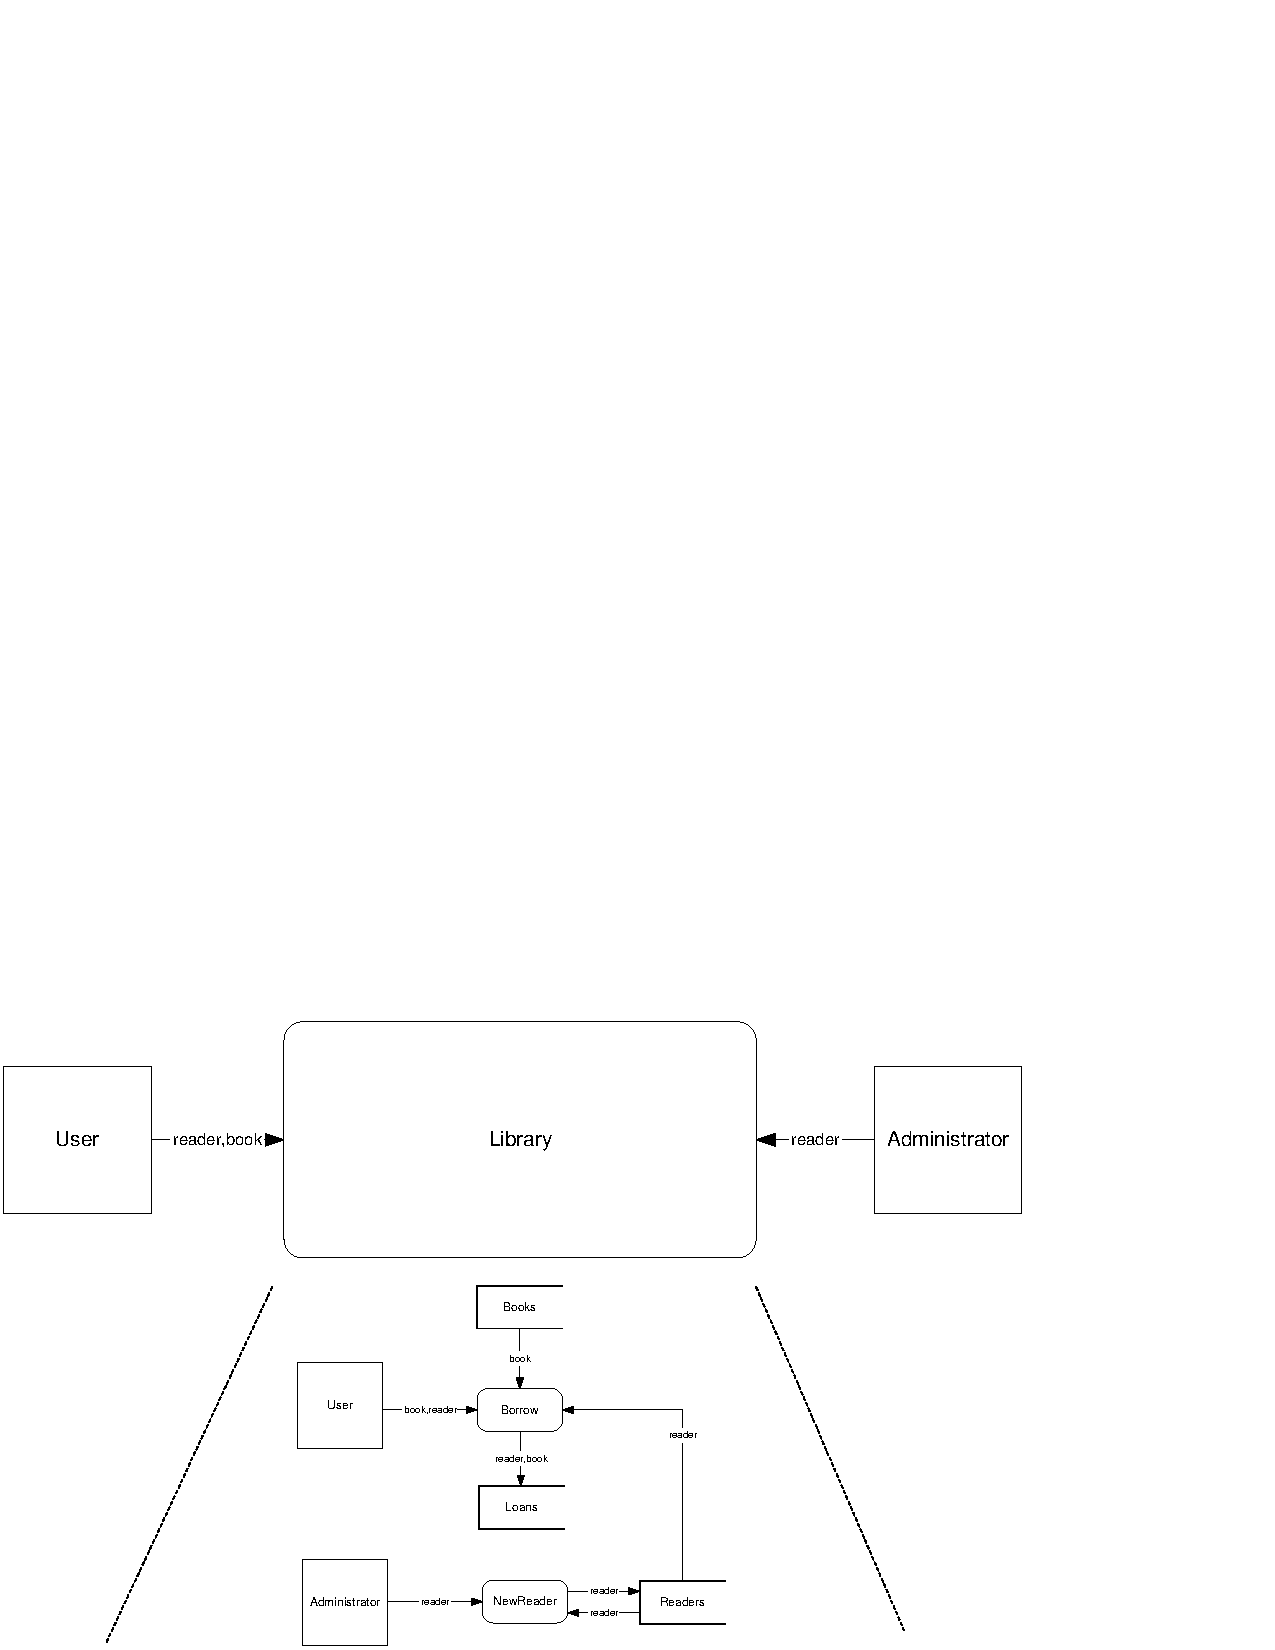
\includegraphics[width=13cm]{AbstractSyntax/figures/DFDContext.pdf}
\caption{A nested DFD}
\label{dfdnested}
\end{center}
\end{figure}

Processes can be decomposed to any level of detail. The diagram in figure \ref{addreader} shows the decomposition of the NewReader process.

\begin{figure}[htb]
\begin{center}
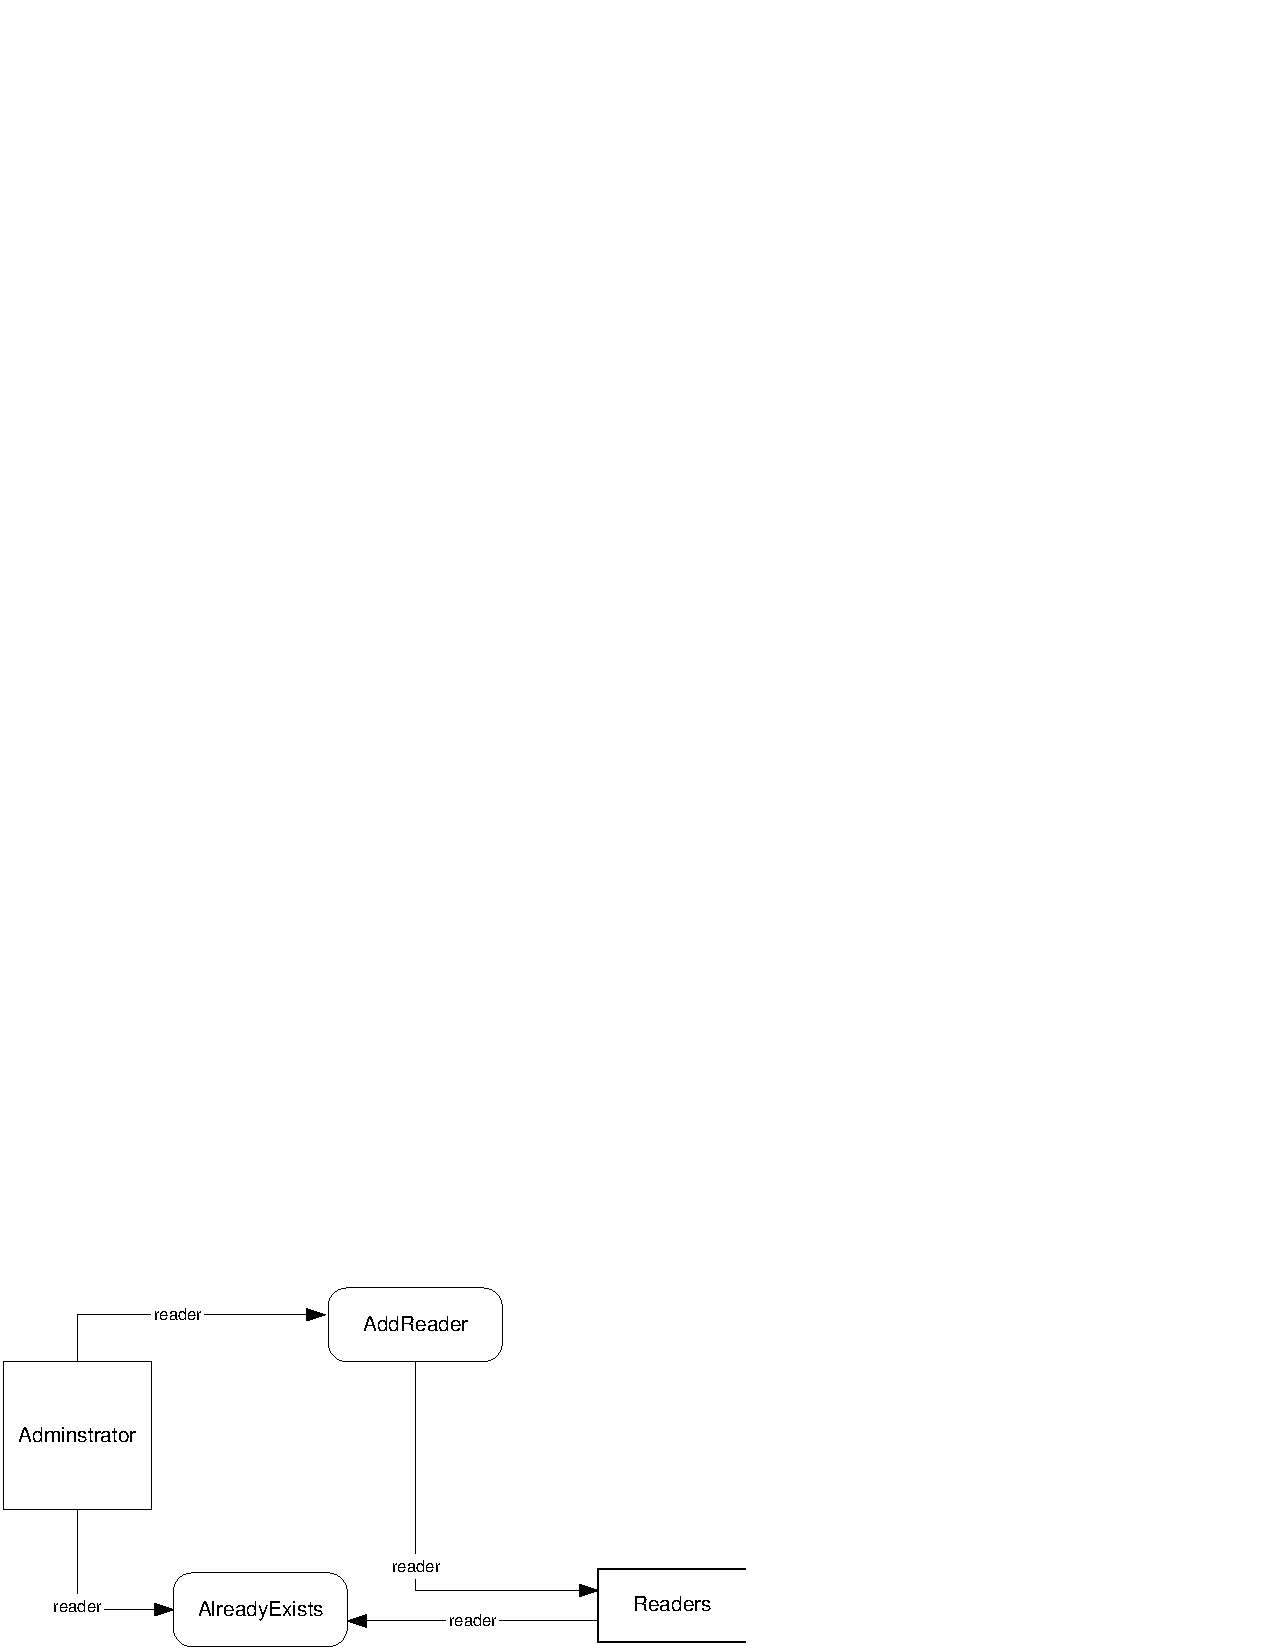
\includegraphics[width=13cm]{AbstractSyntax/figures/AddReader.pdf}
\caption{Decomposing the NewReader process}
\label{addreader}
\end{center}
\end{figure}

Finally, in order to describe the effect of a leaf process, DFDs typically provide a simple action language. This can be a specification style language, such as Pspecs \cite{}, which describes the effect of the process in terms of pre- and post- conditions, or it can be an operational language. Because we ultimately wish to be able to execute the DFD's, the latter has been chosen. 

The action language supports a collection of simple actions for updating and reading records from datastores, making choices, and calling other actions in other processes.

\small
\begin{verbatim}
@Process AddReader(name)
  @When
    not Readers.records->exists(reader | reader->at(0) = name) 
  do
    @Block
      @Update Readers with Seq{name} end
      @OCLExp "ReaderAdded" end
    end
  end
end
\end{verbatim}
\normalsize    

The action illustrated here is a When action, which has a condition, that, if true, results in the activation of the action in the do expression. In this case, if no reader currently exists with the same name in the Readers datastore, a sequential Block action is called. This firstly updates the Readers datastore with a sequence containing the name of the reader and then produces the OCL string expression, "ReaderAdded".   

\subsection{Identification of Concepts}

Based on the example shown in figure \ref{dfdexample}, the following candidates for concepts can be immediately identified:

\begin{description}
\item [Process]  A transformer of information that resides within the bounds of the system to be modelled. Processes appear as named circles in a DFD.

\item [External Entity] A producer or consumer of information that resides outside the bounds of the system to be modelled. An external entity is drawn as a named box.

\item [Datastore] A repository of data records that is to be stored for use by one or more processes. A datastore is drawn as a half open box.

\item [Dataflow] Represents the flow of data between processes, entities and datastores. Dataflows are named and are uni-directional. Dataflows are shown as lines with a single arrow at one end, pointing in the direction of the flow.

\item [Action] An action belongs to a process and has a body which specifies the effect of the action. The following primitive sets of actions are provided: 
\begin{itemize}
\item A Send action causes a process in scope to be activated by sending the process a message.
\item An Update action is used to add a record to a data store.
\item A Remove action removes a record from a datastore.
\item An Or action performs a number of actions in sequence until one of them succeeds. 
\item A When action allows actions to be activated provided a condition holds.
\item A Block action contains a sequence of sub-actions, which are activated in order.
\item An OCLExp action that contains an XOCL expression which can be evaluated in the normal way.
\end{itemize}

\end{description}

Figure \ref{dfdannotated} shows the same DFD model 'marked up' with some of the identified concepts. A similar exercise can be carried out for elements in the action language example.

\begin{figure}[htb]
\begin{center}
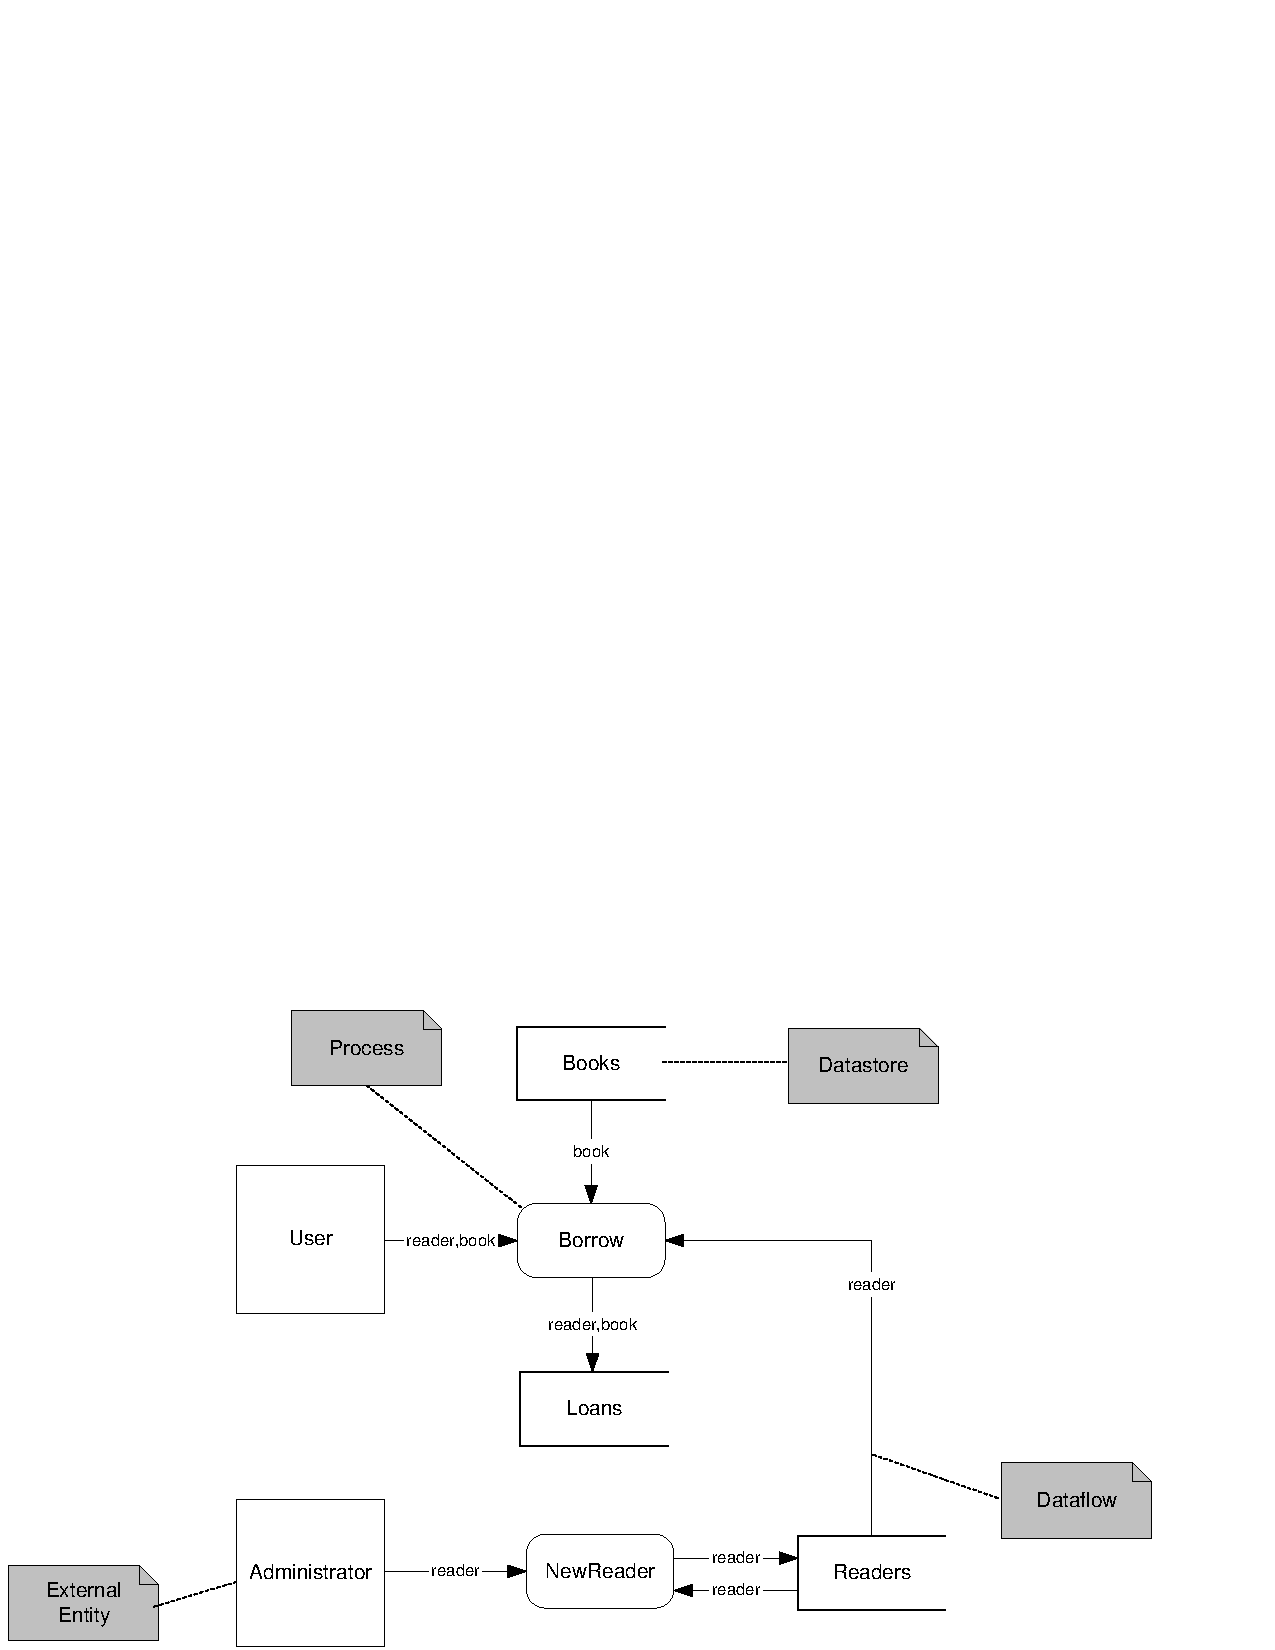
\includegraphics[width=13cm]{AbstractSyntax/figures/DFDAnnotated.pdf}
\caption{An annotated example of a data flow diagram (DFD)}
\label{dfdannotated}
\end{center}
\end{figure}

\subsection{The Model}

Once some candidate concepts have been identified, the next step is to construct the model. 

An important question to ask at this point is whether each concept is an appropriate abstract syntax concept. Datastores, processes and actions are clearly core to DFDs, as they capture the central concepts of data and data transformation. There is a question mark however over external entities and data flows:

\begin{itemize} 
\item External entities are external to the system being modelled, and would appear to be redundent in the sense that they only add contextual information. \item Dataflows appear to be derived concepts, as they could be thought of as showing information flow dependencies between processes and datastores as the result of actions. For instance, a flow from a process to a datastore can be derived from an action belonging to the process that updates the datastore.
\end{itemize}

\noindent For now, these two concepts will be put to one side \footnote{They will be considered further in the concrete syntax chapter}. 

By focusing on processes, datastores and actions, the model shown in figure \ref{dfdabs1} is obtained.

\begin{figure}[htb]
\begin{center}
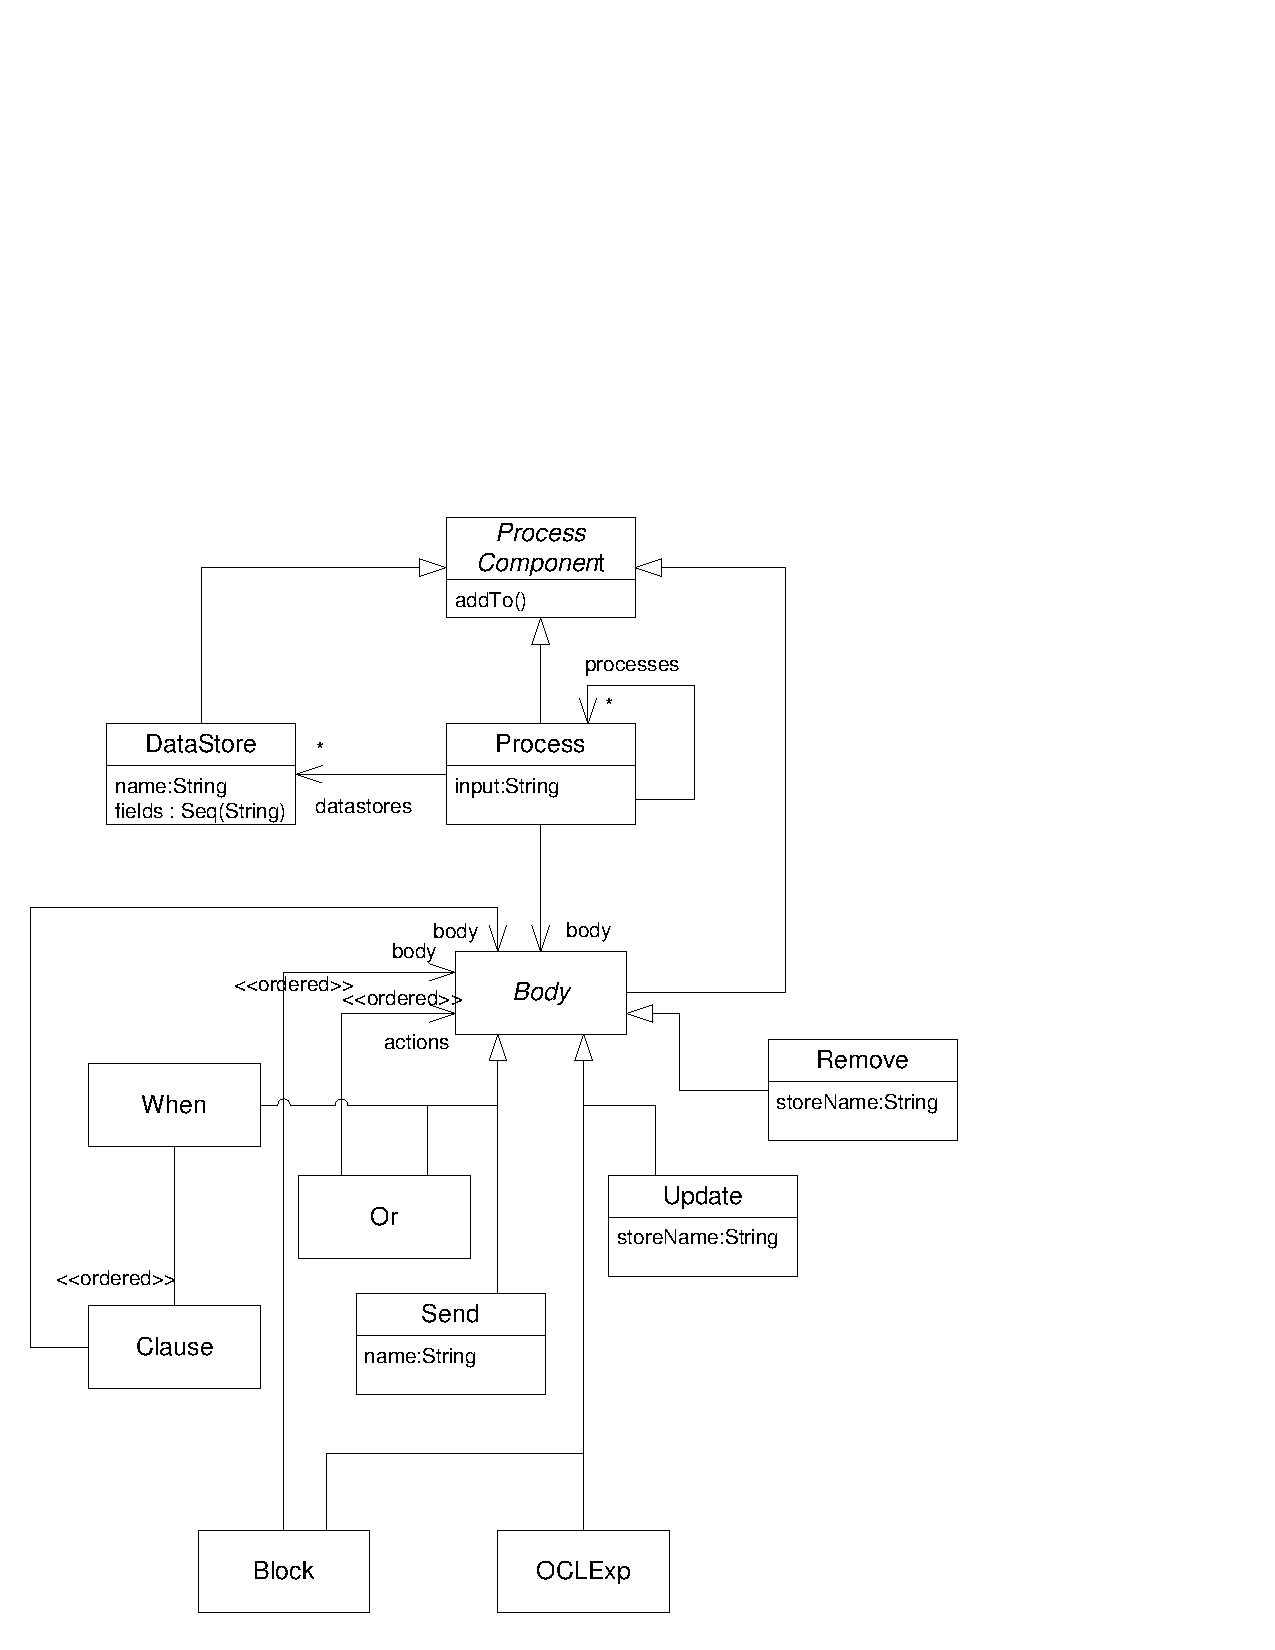
\includegraphics[width=10cm]{AbstractSyntax/figures/DFDAbs1.pdf}
\caption{An bstract syntax metamodel for DFDs}
\label{dfdabs1}
\end{center}
\end{figure}

There are a number of points to note about the model:

\begin{itemize}
\item Processes are associated with: the collection of datastores that are accessible by the process; a single action body; and the collection of sub-processes belonging to the process. A process has a single 'argument' that it uses to refer to input messages. The body of the process provides its output messages.
\item Datastores contain an attribute, fields, which defines the names of the elements in each of its records.
\item Any element that can be viewed as a component of a process is a specialisation of the class ProcessComponent. This provides an abstract operation, addTo(), which defines how a component adds itself to a process.
\item {\it When} expressions are associated with a collection of clauses, which define the rules for testing whether the body of the clause should be activated.
\end{itemize}

\subsection{Well-formedness Rules}

Whilst most of the concepts and relationship in the DFD language have been identified,  there are some important rules missing about what constitutes a well-formed DFD. Firstly, it must be the case that sub-processes and datastores associated with a process have unique names:

\small
\begin{verbatim}
context Process
@Constraint AllProcessesHaveUniqueNames
  processes->forAll(p1 |
    processes->forAll(p2 |
      p1.name = p2.name implies p1 = p2))
end

context Process
@Constraint AllDataStoresHaveUniqueNames
  dataStores->forAll(p1 |
    dataStores->forAll(p2 |
      p1.name = p2.name implies p1 = p2))
end
\end{verbatim}
\normalsize

Finally, there are some rules relating to nesting:

\begin{enumerate}
\item There should be no cyclic nesting of processes. This is required in order to avoid there being cyclic dependencies in a DFD.
\item Sub-processes must only have access to datastores that are accessible by their parent processes.
\end{enumerate}

\noindent These rules can be expressed as follows:

\small
\begin{verbatim}
context Process
@Constraint NoCyclicDependencies
  not self.allOwnedProcesses()->includes(self)
end  

context Process
@Constraint DatastoresAreInherited
   datastores->includesAll(processes.datastores)
\end{verbatim}
\normalsize

\noindent Where the definition of the operation allOwnedProcesses() is given by the following OCL expression:

\small
\begin{verbatim}
context Process
@Operation allOwnedProcesses():Set(Process)
  processes->
    collect(p | p.allOwnedProcess())
end  
\end{verbatim}
\normalsize

\subsection{Operations}

The following operations are defined for a process:

\small
\begin{verbatim}
context Process
@Operation addTo(p:Process)
  p.addProcess(self)
end

context Process
@Operation addStore(store:DataStore)
  self.dataStores := dataStores->including(store)
end

context Process
@Operation addProcess(process:Process)
  self.processes := processes->including(process)
end 
\end{verbatim}
\normalsize

The operation addTo() adds a process as a sub-process to the current process by calling the addProcess() operation. The addStore() operation adds a datastore to the collection of datastores that are accessible by the process.

The operation addTo() is similarly defined for a datastore:

\small
\begin{verbatim}
@Operation addTo(p:Process)
  p.addStore(self)
end
\end{verbatim}
\normalsize

As we shall see in chapter ??, these operations will become useful when populating DFDs during parsing.

\subsection{Validating the DFD metamodel}

In figure \ref{dfdsnapshot} a partial object diagram corresponding to the DFD in figure \ref{dfdexample} is shown. Here, instances of XOCL expressions are the values that are passed as expressions to the actions. The main point to note about this diagram is that it satisfies the well-formedness rules of the DFD. 

\begin{figure}[htb]
\begin{center}
\includegraphics[width=10cm]{AbstractSyntax/figures/DFDsnapshot.pdf}
\caption{An object diagram corresponding to figure \ref{dfdexample}}
\label{dfdsnapshot}
\end{center}
\end{figure}

However, this is about as far as we can go. At this point, the model is just a model of the abstract syntax and nothing more. To enable DFDs to be conveniently inputed, parsed and executed both the concrete syntax and semantics of the language must be modelled too. These aspects will be explored in the following chapters. 

\section{Conclusion}

This chapter has examined the process and modelling language required to model the abstract syntax of languages. The result is a definition of the concepts in a language and the relationship and rules that govern them. However, this is just a first step towards a complete definition of the language. Only once the concrete syntax and semantics of the language are modelled does it become a true metamodel.

